\documentclass[12pt, a4paper]{article}
\usepackage[top=2cm, bottom=2cm, left=2cm, right=2cm]{geometry}
\usepackage{amsmath,amsfonts,amssymb}
\usepackage{indentfirst,enumitem}
\usepackage{graphicx}
\usepackage[font=small,labelfont=bf]{caption}
\usepackage{multicol}
\usepackage{setspace}
\usepackage{hyperref}
\usepackage{listings}
\usepackage{tabularx}
\usepackage{hyperref}
\usepackage[dvipsnames]{xcolor}
\usepackage{scrextend}
\usepackage{comment}
\usepackage{soul}
\usepackage{tikz,tkz-tab}
\usepackage{lscape}
\usepackage{float,lscape}
\usepackage{fancyhdr}
\usepackage{tcolorbox}
\usepackage{titling}
\usepackage{import}
\usepackage{titlesec}
\usepackage{color}

%\changefontsizes{13pt}

%New colors defined below
\definecolor{codegreen}{rgb}{0,0.6,0}
\definecolor{codegray}{rgb}{0.5,0.5,0.5}
\definecolor{codepurple}{rgb}{0.58,0,0.82}
\definecolor{backcolour}{rgb}{0.95,0.95,0.92}

\hypersetup{
    colorlinks=true,% make the links colored
}

%Code listing style named "mystyle"
\lstdefinestyle{mystyle}{
  backgroundcolor=\color{backcolour},   commentstyle=\color{codegreen},
  keywordstyle=\color{blue},
  numberstyle=\tiny\color{codegray},
  stringstyle=\color{codepurple},
  basicstyle=\ttfamily\footnotesize,
  breakatwhitespace=false,
  breaklines=true,
  captionpos=b,
  keepspaces=true,
  numbers=left,
  numbersep=5pt,
  showspaces=false,
  showstringspaces=false,
  showtabs=false,
  tabsize=2
}

%"mystyle" code listing set
\lstset{style=mystyle}

\begin{document}
\begin{titlepage}
%\SetWatermarkText{\includegraphics[width = 0.97\paperwidth,
%height = 0.97\paperheight]{bia.png}}
%\SetWatermarkAngle{0}
%\SetWatermarkText{\includegraphics[scale=1]{hust.png}}
%\SetWatermarkAngle{0}
\begin{tikzpicture}[remember picture,overlay,inner sep=0,outer sep=0]
     \draw[blue!70!black,line width=4pt] ([xshift=-1.5cm,yshift=-2cm]current page.north east) coordinate (A)--([xshift=1.5cm,yshift=-2cm]current page.north west) coordinate(B)--([xshift=1.5cm,yshift=2cm]current page.south west) coordinate (C)--([xshift=-1.5cm,yshift=2cm]current page.south east) coordinate(D)--cycle;

     \draw ([yshift=0.5cm,xshift=-0.5cm]A)-- ([yshift=0.5cm,xshift=0.5cm]B)--
     ([yshift=-0.5cm,xshift=0.5cm]B) --([yshift=-0.5cm,xshift=-0.5cm]B)--([yshift=0.5cm,xshift=-0.5cm]C)--([yshift=0.5cm,xshift=0.5cm]C)--([yshift=-0.5cm,xshift=0.5cm]C)-- ([yshift=-0.5cm,xshift=-0.5cm]D)--([yshift=0.5cm,xshift=-0.5cm]D)--([yshift=0.5cm,xshift=0.5cm]D)--([yshift=-0.5cm,xshift=0.5cm]A)--([yshift=-0.5cm,xshift=-0.5cm]A)--([yshift=0.5cm,xshift=-0.5cm]A);


     \draw ([yshift=-0.3cm,xshift=0.3cm]A)-- ([yshift=-0.3cm,xshift=-0.3cm]B)--
     ([yshift=0.3cm,xshift=-0.3cm]B) --([yshift=0.3cm,xshift=0.3cm]B)--([yshift=-0.3cm,xshift=0.3cm]C)--([yshift=-0.3cm,xshift=-0.3cm]C)--([yshift=0.3cm,xshift=-0.3cm]C)-- ([yshift=0.3cm,xshift=0.3cm]D)--([yshift=-0.3cm,xshift=0.3cm]D)--([yshift=-0.3cm,xshift=-0.3cm]D)--([yshift=0.3cm,xshift=-0.3cm]A)--([yshift=0.3cm,xshift=0.3cm]A)--([yshift=-0.3cm,xshift=0.3cm]A);

   \end{tikzpicture}
    
\begin{center}
    
\includegraphics[width = 0.5\textwidth]{./image/3.png}
\end{center}
\vspace{10pt}
\begin{center}

    \vspace{10pt}
    \fontsize{18pt}{17pt}\selectfont
    \textbf{TEAM: ROBOTRONIX}

    \vspace{7pt}
    \textbf{GROUP: C++}
\end{center}


\vfill
\centerline{\bf Ho Chi Minh city - 2024}
\vspace{0.5cm}
\end{titlepage}
\newpage
\thispagestyle{empty}
\textbf{Team information}

\textbf{Group}: C++

\textbf{Team name}: ROBOTRONIX

\textbf{Guidance teacher}: Nguyen Thi Thuy Hanh

\textbf{Team members}:\\

\begin{tabularx}{1\textwidth} { 
    | >{\raggedright\arraybackslash}X 
    | >{\raggedright\arraybackslash}X  |}
   \hline
   \textbf{Full name} & \textbf{University} \\ \hline
    Nguyen Dang Hoai Nam & UEL \\ \hline
    Le Minh Nguyen & UEL \\ \hline
    Bui Nguyen Thanh Thao & UEH \\ \hline
    Vu Nhat Huy & HCMUT \\ \hline
    Tran Xuan Hao & HCMUT \\ \hline
    Vu Hoang Tung & HCMUT \\ \hline
  \end{tabularx}
\newpage
\thispagestyle{empty}
{
  \hypersetup{linkcolor=[RGB]{0, 0, 0}}
  \tableofcontents
}
\onehalfspacing
%%%%%%%%%%%%%%%%%%%%%%%%%%%%%%%%%%%%%%%%%%%%%%%%%%%%%%%%%%%%%%%%%%%%%%%
\newpage
\setcounter{page}{1}
\section{Introduction}
This project proposes the use of the Yanshee robot to modernize various aspects of life. Robots are increasingly used in business for decision-making and work automation and in homes for tasks like weather forecasting and object recognition. Our team, using Agile methodology, has developed features for the compact Yanshee robot, such as object recognition and weather information retrieval. This contributes to household modernization and business management by providing data access and management, reducing decision-making time, avoiding risks, and enhancing user experience.
%%%%%%%%%%%%%%%%%%%%%%%%%%%%%%%%%%%%%%%%%%%%%%%%%%%%%%%%%%%%%%%%%%%%%
\section{Deploying Yanshee}
\subsection{Gemini Assistant}
Applying one of the most popular Large Language Models - Gemini. We've been rigorously evaluating Yanshee's performance on a wide variety of tasks. From natural image, audio, and video understanding. 
\subsection{Weather API Integration}
This function allows accessing and retrieving weather data, such as current temperature, pressure, and weather descriptions via an Application Programming Interface (API). This data is commonly used in digital applications and web platforms, but its integration into robotics offers a promising research and development area. For instance, we decided to enable Yanshee to access real-time weather information to enhance its user interaction functionalities.
\subsection{Object Detection}
It is a computer vision technique for locating instances of objects in images or videos. This technology when applied to Yanshee has various applications in human interaction, decision-making under different environments, and completing tasks, particularly in teaching children, …
\subsection{Facial Recognition}
Facial recognition when applied in robots can open up opportunities in social interactions. By recognizing faces, and hearing voices, the robot can be used in therapy, guidance, and identifying threats with close intimacy and personalized experience with specified users.
\subsection{Dancing and Playing Music}
We programmed Yanshee to play the user's favorite music. Moreover, Yanshee can perform dances based on your favorite music.
\subsection{Instruction}
\begin{center}
    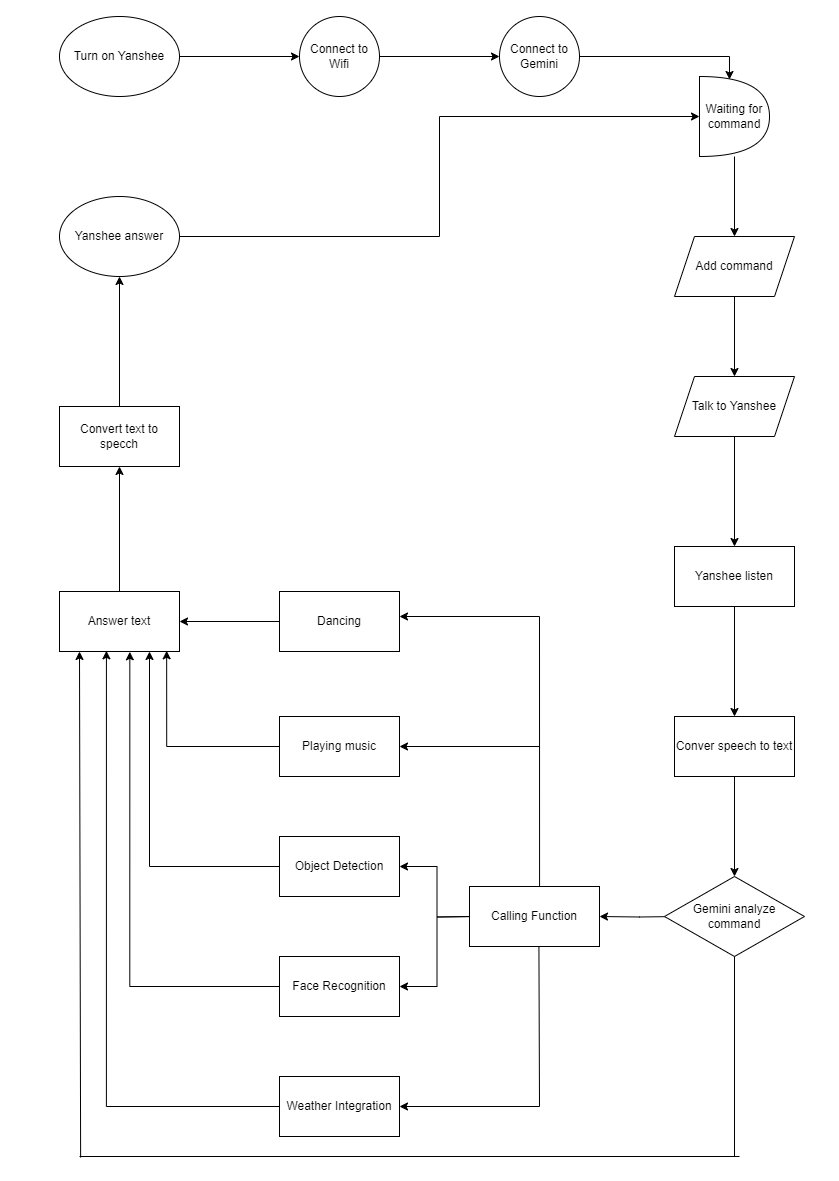
\includegraphics[width = 0.65\textwidth]{./image/4.png}
\end{center}
\begin{itemize}
    \item[-] \textbf{Gemini Assistant:}
\end{itemize}

Firstly, we need to turn on the robot by holding the button on Yanshee's chest. We must make sure that Yanshee and remote access device are connected to the same Wifi network. After finishing, Yanshee will become your friendly assistant. Users must be careful to avoid misspelling or mispronouncing. This may lead to the situation Yanshee misunderstand your command.

\begin{itemize}
    \item[-] \textbf{Weather API Integration:}
\end{itemize}

To have the weather information in a specific city, you need to give commands to Yanshee such as “Can you give me the weather information in New York?” or “What is the weather like today in New York?”. Yanshee will listen and find the weather information in New York and generate an answer for you.

\begin{itemize}
    \item[-] \textbf{Object Detection:}
\end{itemize}

Yanshee's object detection capabilities are designed as two distinct approaches, each yielding different outcomes to serve distinctive purposes: one advanced Gemini to produce natural human text; the other emphasizes precise object labeling for effective real-time action monitoring and AI-driven decision-making, suitable for circumstances requiring precision and speed. These methods enable Yanshee to serve diverse purposes, from improving human-robot interactions to executing complex tasks with real-time accuracy and reliability.
\begin{figure}[h!]
    \centering
    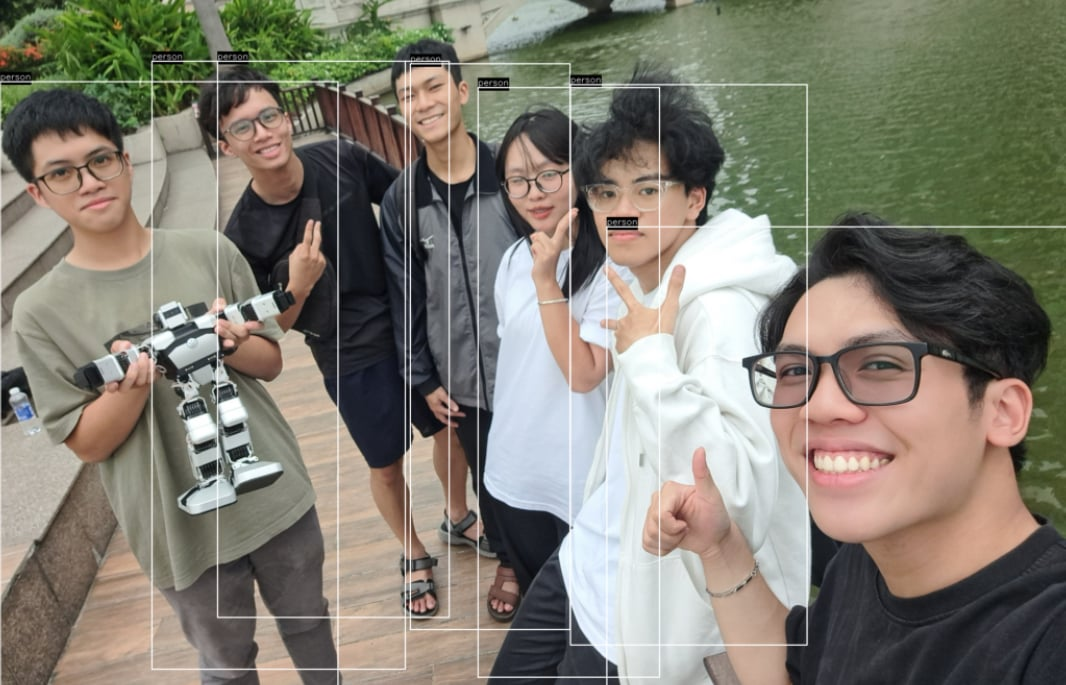
\includegraphics[width=7.5cm]{./image/5.png}
    \qquad
    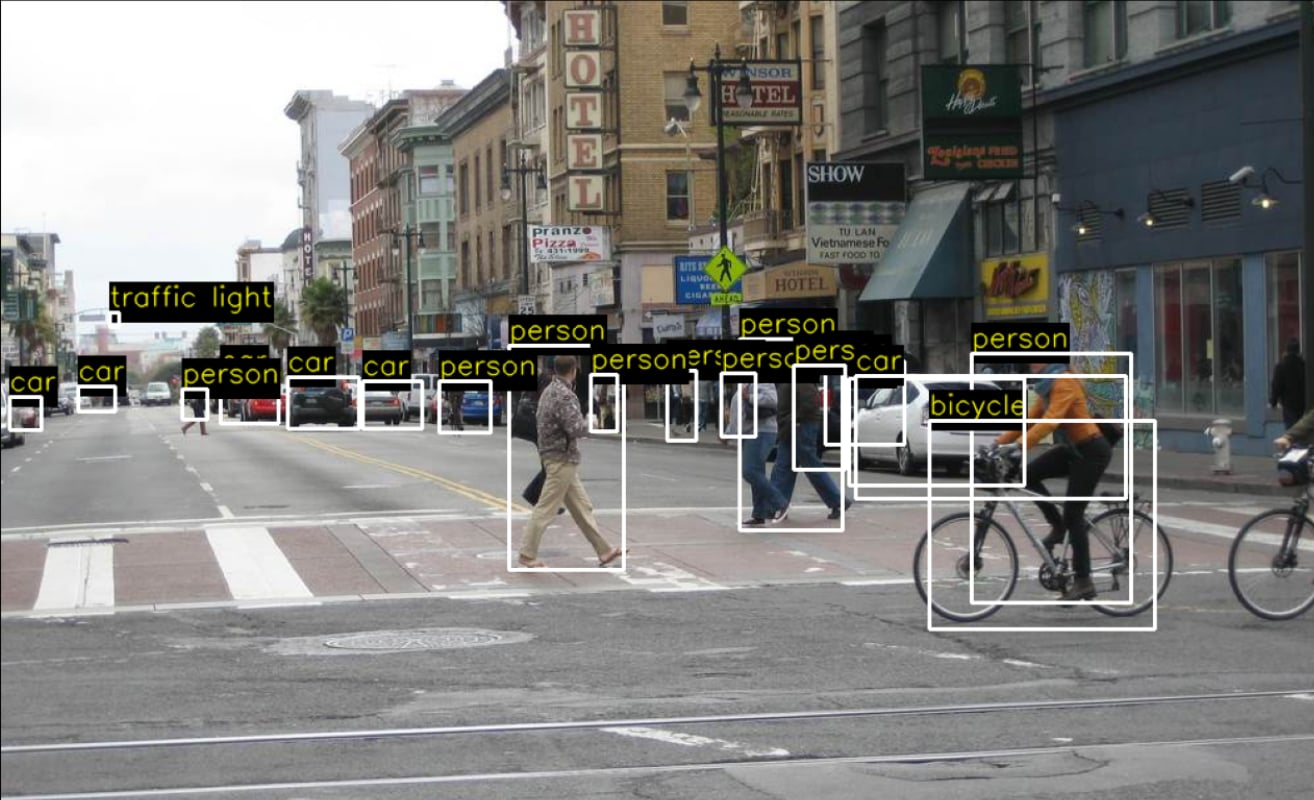
\includegraphics[width=7.5cm]{./image/2.png}
\end{figure}

During interactions, Yanshee will use object detection to analyze its surroundings. When users ask questions like "What is in front of us?" or "How is the view?", Yanshee takes a picture of the view and uses Gemini to produce human-understandable text, which is then converted to speech. This enhances human interaction and serves target users such as children and disabled people. For example, it can tell a blind person what is in front of them or warn children of dangerous objects like knives and cars. Input pictures are planned to be taken every 0.5 seconds or under certain conditions and events, such as receiving tasks to find and pick up objects. These inputs are sent to our object-detection model to swiftly generate precise labels and format them as computer-readable data, making the process faster and more efficient for the robot to handle.
\begin{itemize}
    \item[-] \textbf{Facial Recognition:}
\end{itemize}

During interactions, Yanshee employs facial recognition to capture what it sees. When users ask questions like “Who do you see?” or “Do you recognize me?”, Yanshee captures the image in front of it and utilizes the Gemini method and the facial recognition method to generate human-understandable text, which is then converted into speech correspondingly to the user it recognizes, eg, “Hello Nam” in the case it recognizes the user is Nam. Users can also load unknown face data to the facial recognition model via commands such as “Add this person you see to your face data.” and it will prompt Yanshee to learn the designated face. This capability greatly enhances human interactions and benefits target users such as children and individuals with disabilities.
\begin{itemize}
    \item[-] \textbf{Dancing and playing music:}
\end{itemize}

To activate the “Playing music” feature, you need to ask Yanshee such as “I want to listen to music.”, “Can you play music?”, etc. Yanshee will generate your command to text and analyze it. Then Yanshee will reply “What song can I play for you?”. Now you can give the song information like name for Yanshee. For instance, “I want to play Taste.”, Yanshee will find the song in its system. If it already exists, Yanshee will turn on that song. Else Yanshee will search on online applications to download and play that song for you. 

Yanshee is also developed to dance to specific songs, our team gave Yanshee the ability to dance. For example, Yanshee can play music and perform dance hits such as “Wakawaka '' or “Sorry Sorry”.
%%%%%%%%%%%%%%%%%%%%%%%%%%%%%%%%%%%%%%%%%%%%%%%%%%%%%%%%%%%%%%%%%%%%%
\section{During Deploying Process}
\subsection{Advantages}
We're able to work with Yanshee to develop this robot to be more useful and friendly to people. In the development process, we found out that Yanshee can become an artificially intelligent assistant thanks to its Wifi connection. Moreover, the Gemini AI is a Python open-source module that everyone can download and connect just by calling their Open API or importing the modules in the source code.

Yanshee is equipped with a built-in camera that can take photos, and upload them onto its local machine storage. 

Yanshee has been given very beautiful movements by  UBTech. The operating system also has very popular music installed and can play and perform those songs at any time.
\subsection{Disadvantages}
Yanshee has no available method to upload the image from its storage to our personal computers (where the image is processed). Thus, we get the photo from another source. Furthermore, a lot of AI models including object-detection require libraries that are not supported by the system of Yanshee.

Yanshee's music list is very small and if you want to listen to your favorite songs. A program must be written to save the music that the user wants to download so that Yanshee can be commanded to play that music. We also realized we could not directly upload songs from our system to Yanshee's operating system, we had to simultaneously access websites or applications to download songs and directly save downloaded songs to Yanshee's system.
\subsection{Solutions}
Through deeper research, we found a function that allows us to get access to Yanshee's vision. The robot is already equipped with a webcam that can stream (real-time) via HTTP URL: “http://(robotIPaddress):8000/stream.mjpg”. But to extract the images, we must implement them ourselves. Furthermore, we have the best use we could out of the latest Gemini model of Google. Our approach is taking screenshots via the video stream and using those screenshots to process and identify both faces and objects. 

Thanks to modern music applications, we have connected Yanshee with music software through API and open-source libraries in Python to connect and download users' favorite music in a simple way and efficiently.
%%%%%%%%%%%%%%%%%%%%%%%%%%%%%%%%%%%%%%%%%%%%%%%%%%%%%%%%%%%%%%%%%%%%%
\section{Implemented Results}
In the implemented results, Yanshee, connected with Gemini AI, has shown the ability to answer most user queries. Gemini's large database and internet access allow it to compile comprehensive answers, providing users with necessary information. This connection with Gemini AI has enabled Yanshee to become a reliable source of information for users.
\begin{center}
    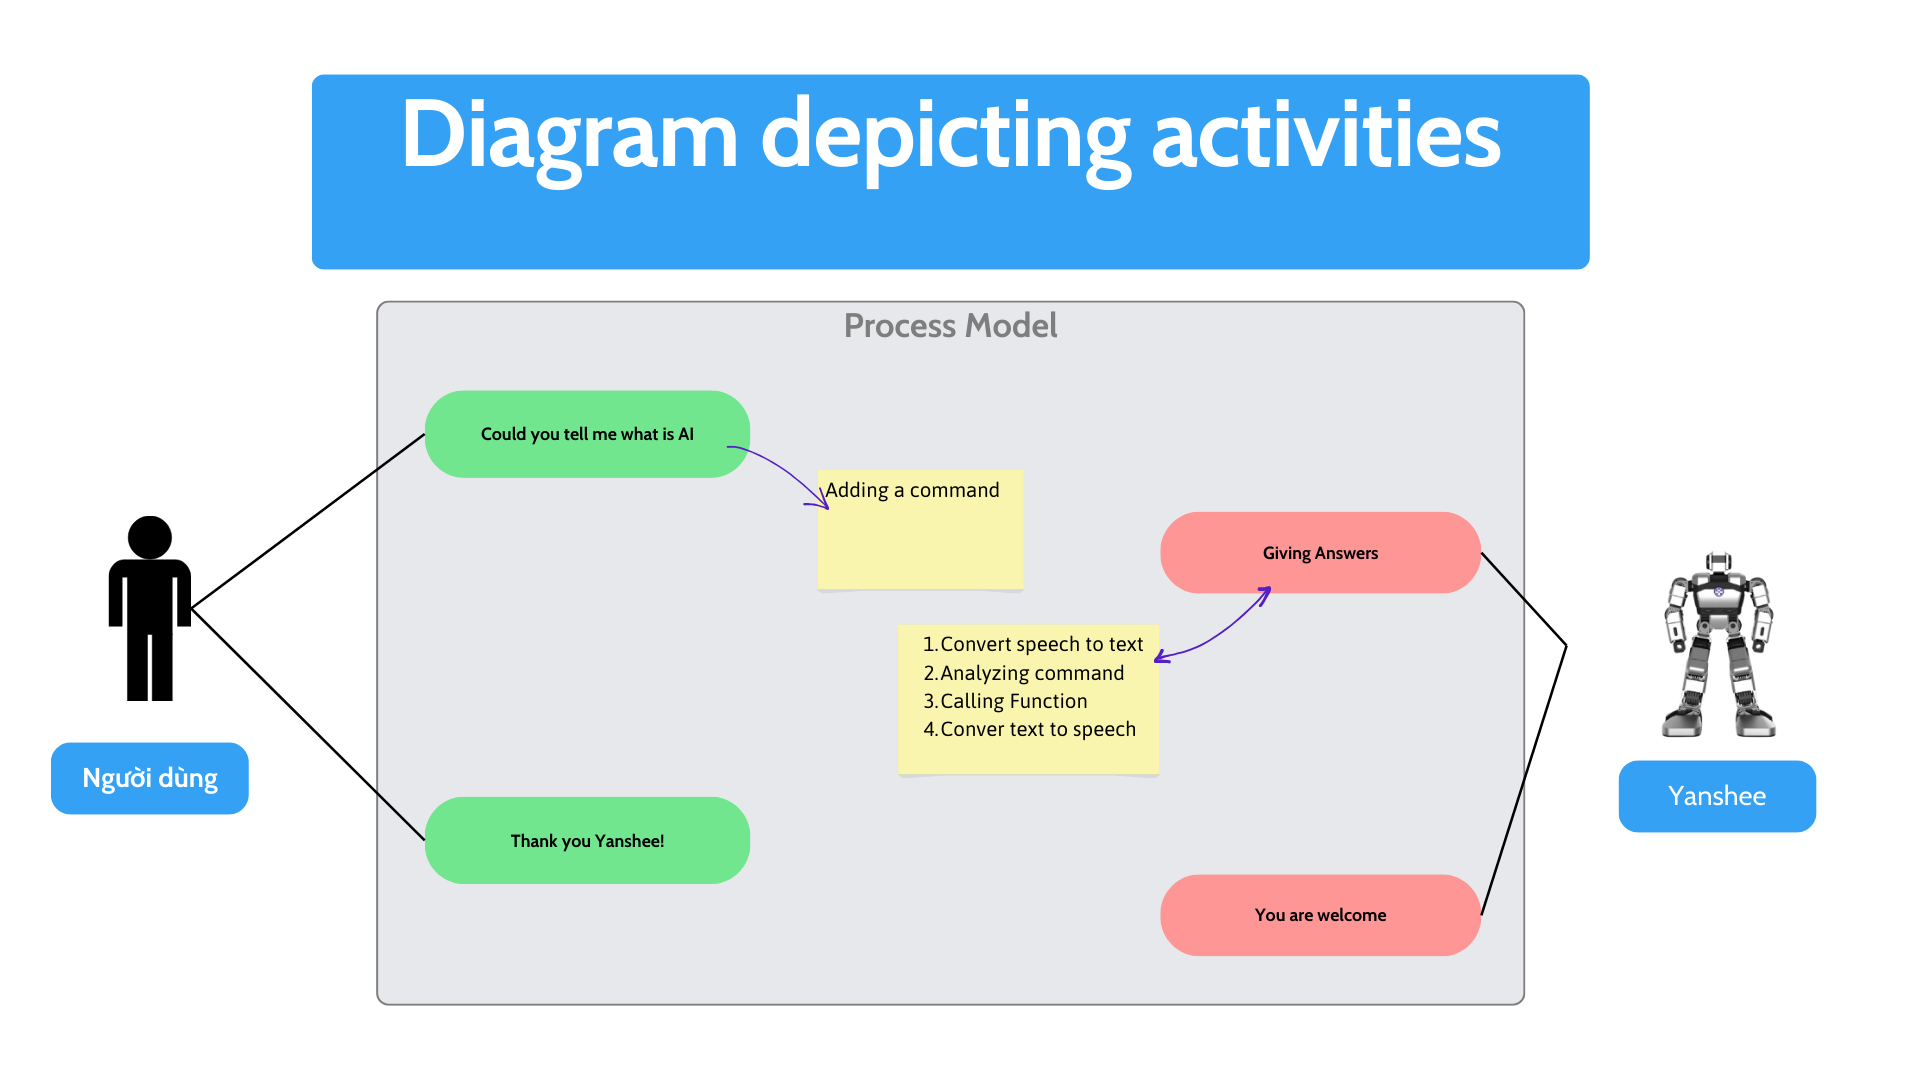
\includegraphics[width = 10cm]{./image/7.png}
\end{center}

To optimize Yanshee's vision capabilities, our team has applied machine learning models to enable Yanshee to learn object and facial recognition. This integration allows Yanshee to analyze and describe images received through its ”eyes.”

In addition to connecting with Gemini via Wi-Fi, we have also integrated connections with reputable weather information websites on the Internet through Wi-Fi. This feature provides users with accurate weather information from around the world, enabling them to plan effectively based on the weather data provided by Yanshee. In addition to weather, Yanshee can find, download, and play music, sometimes even dance to it, a rare feature among robots currently available.
\begin{center}
    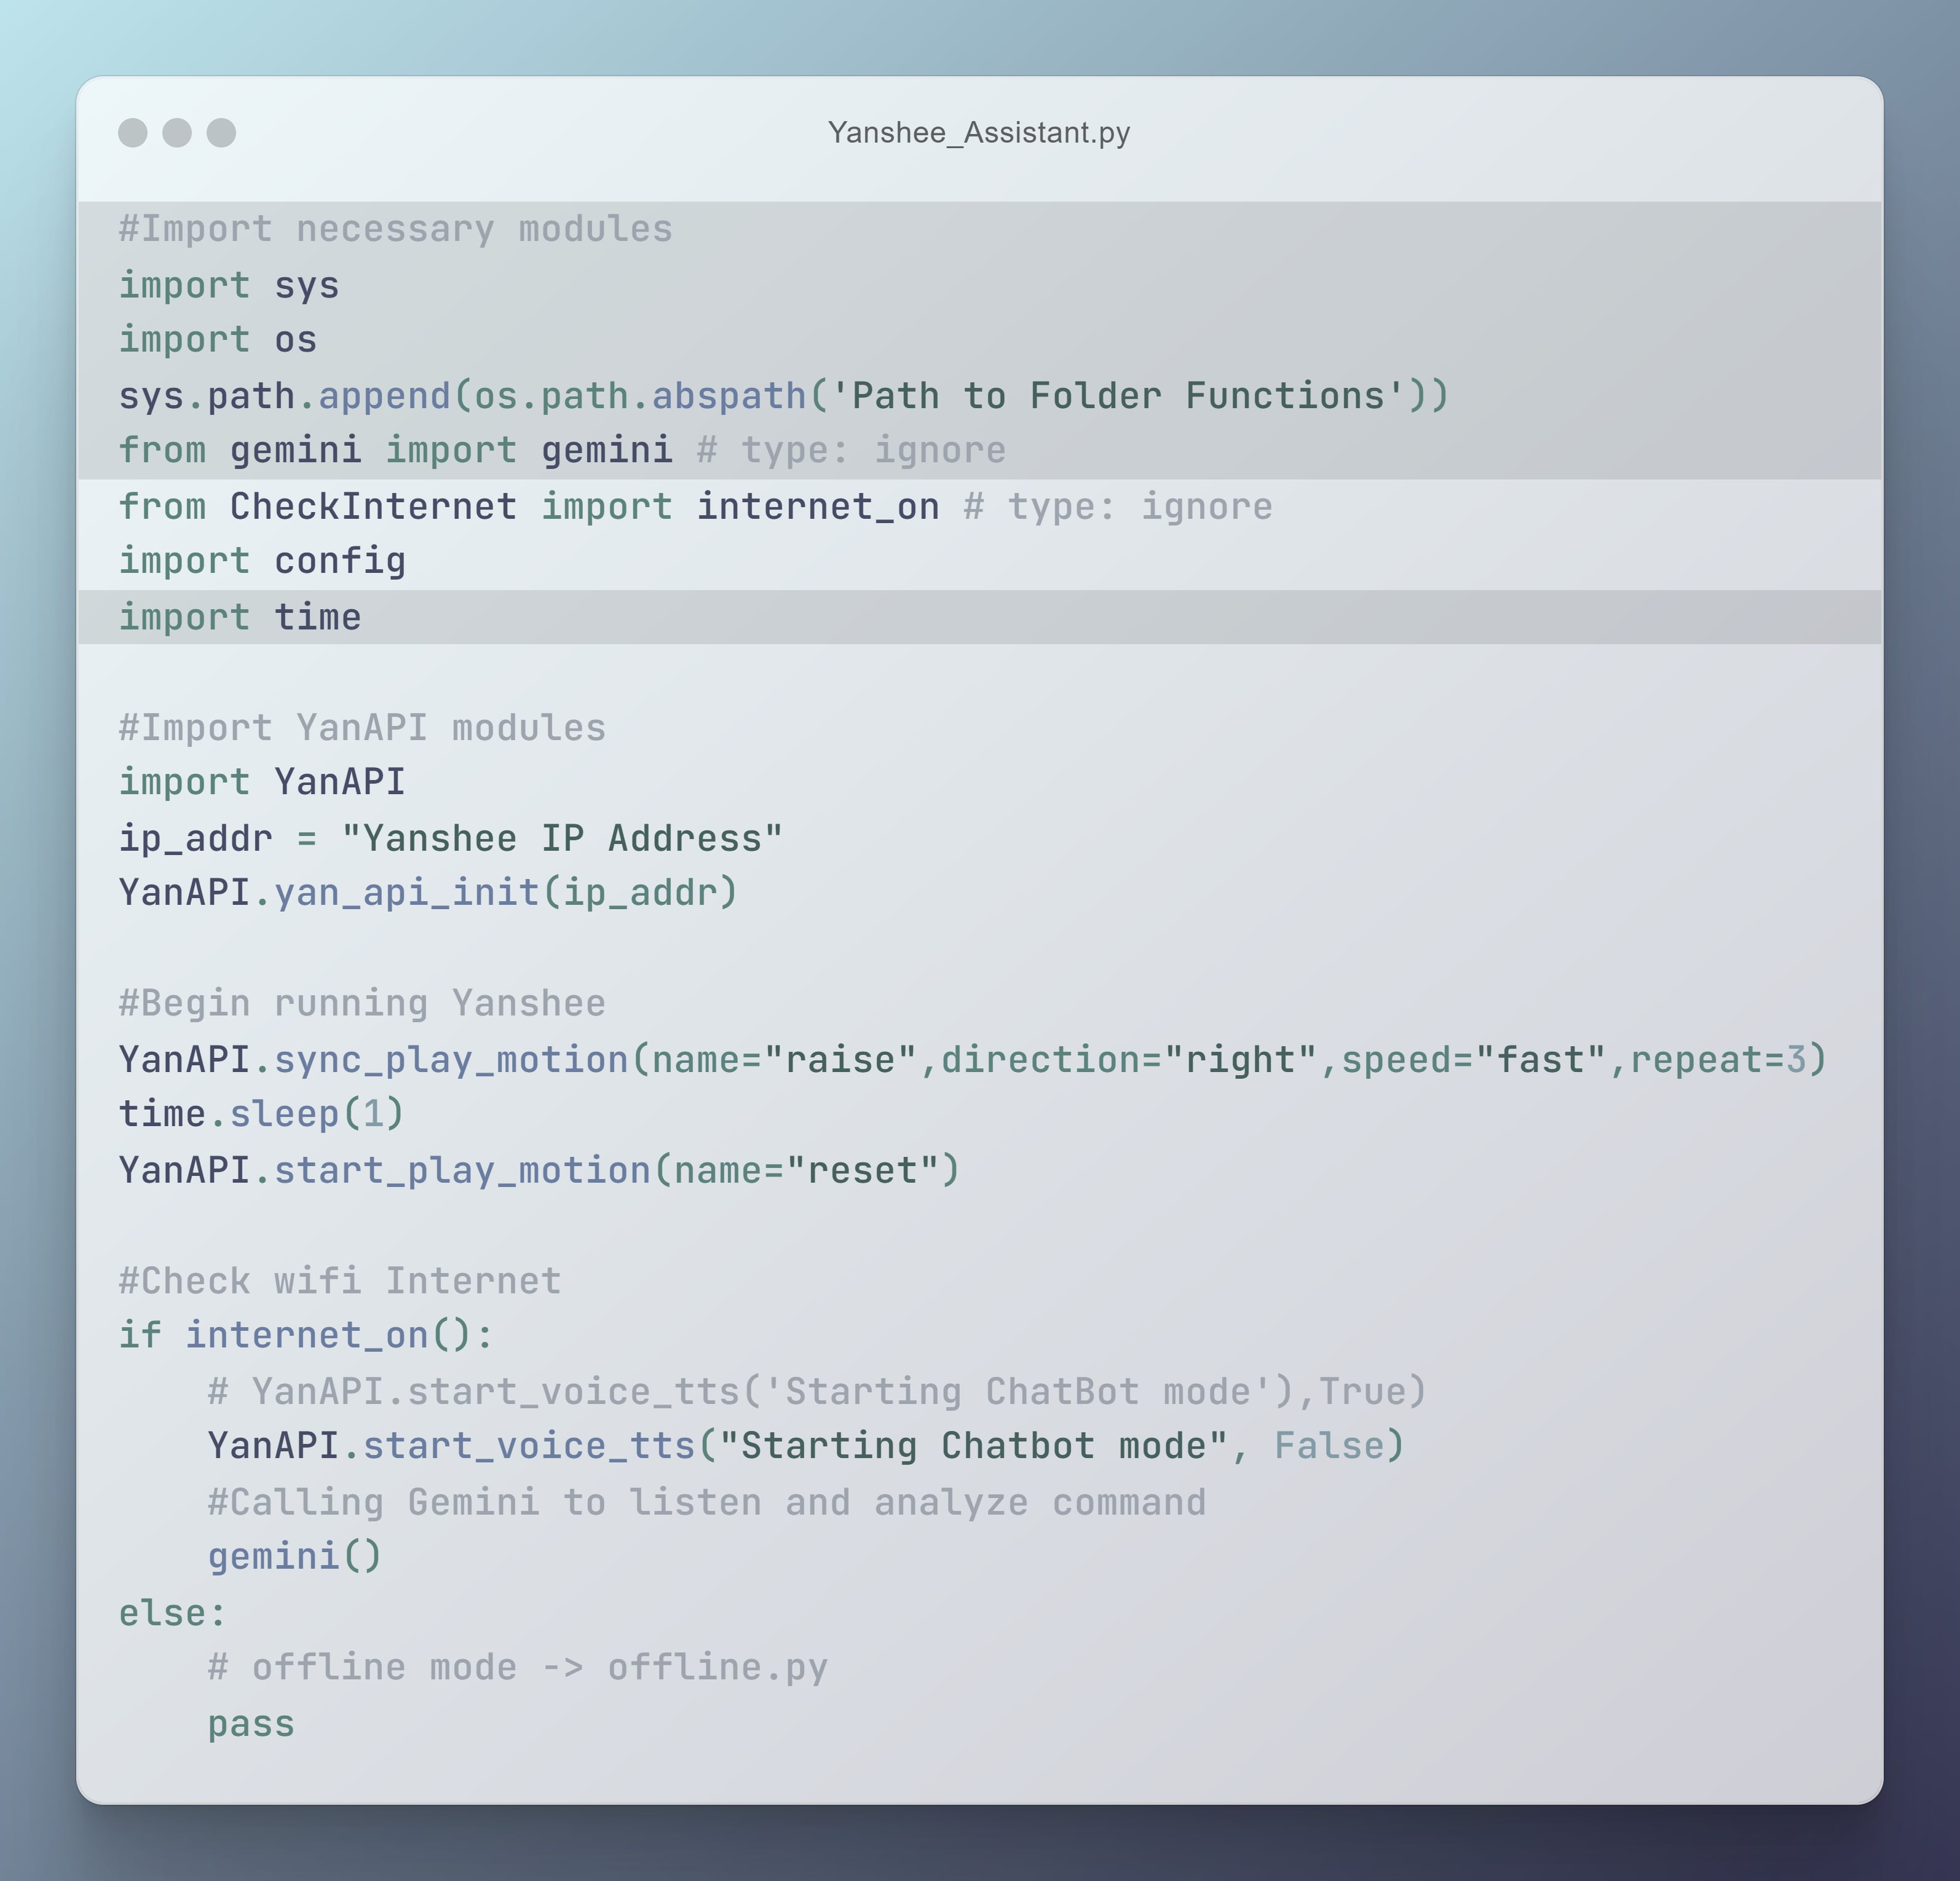
\includegraphics[width = 0.6\textwidth]{./image/6.png}
\end{center}
%%%%%%%%%%%%%%%%%%%%%%%%%%%%%%%%%%%%%%%%%%%%%%%%%%%%%%%%%%%%%%%%%%%%%
\section{Conclusion}
In conclusion, we've delved into the advanced features of modern robotics, such as AI, precision engineering, and system integration. These innovations are set to transform industries like manufacturing, healthcare, agriculture, and domestic services by improving efficiency, accuracy, and safety. Robots are transformative agents capable of handling repetitive tasks, performing complex surgeries, assisting in disaster recovery, and even providing companionship in our daily lives.

The future of robotics depends on collaboration between technologists, policymakers, and the public. By addressing ethical issues and ensuring fair access to robotic technologies, we can build a future where robots significantly improve everyone's quality of life.
\end{document}